\chapter{The Ending of Image}

This chapter follows the sixth Brockwood Park dialogue in \emph{The Transformation of Man}, credited to J. Krishnamurti and preserved through the Krishnamurti Foundation Trust source material, with curation by LazyingArt LLC through Video2Book. No validated blackboard equations, sketches, or usable frame-backed diagrams survive for this lecture. The displayed formulae below are therefore not physics formulae and not extracted board work; they are compact bookkeeping devices for the sequence of the inquiry. We use them to keep the argument clear: transformation is brought down to ordinary life, ordinary life is tested in relationship, relationship exposes image, and image leads to the question of the observer, thought, time, and meditation.

\section{From Transformation To Ordinary Life}

The dialogue begins with the largest possible question: what will change man? More exactly, what can bring about a radical transformation in the total consciousness of a human being? The question is first put to a scientist, but the answer immediately lowers the authority of scientific background for this inquiry. That is the first correction in the lecture. We are not going to derive inward transformation from prestige, expertise, or a specialist vocabulary.

A useful first note is therefore negative:

\begin{equation}
\text{radical transformation}
\not\equiv
\text{expert explanation}.
\end{equation}

This is not a rejection of science. It is a refusal to let science become the wrong authority. The question is not, ``What does a physicist know about consciousness?'' It is, ``Where does this inquiry touch the life that is actually being lived?'' Krishnamurti presses the point by taking the side of the ordinary viewer: the person who goes to the office or factory, who has family conflict, poverty, fatigue, sex, children, disappointment, and very little time. Such a viewer may quite reasonably say: bring it nearer.

The first movement of the lecture is therefore a change of scale. The question of transformation is not abandoned, but it is brought to the point where it can be tested.

\begin{equation}
\text{transformation}
\;\longrightarrow\;
\text{ordinary life}
\;\longrightarrow\;
\text{where can it be touched?}
\end{equation}

The phrase ``ordinary life'' should not be heard as a lowering of seriousness. It is the opposite. If a transformation is real, it must meet the actual structure of misery, time pressure, and relationship. Otherwise it remains outside the listener's field.

\section{Relationship As The Field Of Inquiry}

Bohm proposes the starting point: the problems arising in daily relationship. Krishnamurti accepts the proposal at once. Relationship is the first concrete field because it includes office, factory, home, sex, children, insult, woundedness, disappointment, hope, desire for success, and the endless movement of wanting more.

The lecture now makes a practical reduction:

\begin{equation}
\text{ordinary life}
\;\longrightarrow\;
\text{relationship}
\;\longrightarrow\;
\text{image becomes visible}.
\end{equation}

We begin with relationship because relationship is where consciousness shows itself in action. It is easy to speak abstractly about consciousness; it is harder to see how one actually meets another human being. The source of relationship, as the dialogue unfolds it, is not direct contact but image: an image of myself, an image of you, an image of what you should be in relation to me.

When that image is not confirmed, disappointment and hurt appear. When it is confirmed, pleasure and dependence appear. Either way, the image has entered between people.

\subsection{Question \& Answer}

\paragraph{Question.}
Why begin with relationship rather than with a general doctrine of consciousness?

\paragraph{Answer.}
Because relationship is the working surface of consciousness. If consciousness is filled with images, that fact appears first as demand, hurt, expectation, comparison, fear, dependence, and disappointment in relationship. To begin with relationship is to begin where the image is already acting, not where theory can hide it.

\section{Image As The Block In Relationship}

The dialogue now gives the problem a more precise structure. A person may have an image of security, an image of pleasure, an image of entitlement, an image of what is right, an image of what a wife or husband should do, and an image of how another person should complete one's own sense of self. The image is not a harmless picture. It organizes action.

A compact relationship model is:

\begin{equation}
\text{self-image}
+
\text{image of the other}
+
\text{claim}
\;\longrightarrow\;
\text{forced relationship}
\;\longrightarrow\;
\text{conflict}.
\end{equation}

The important word is ``forced.'' Once the image is active, the other person is no longer simply met. The other is asked, silently or openly, to acknowledge the image. You should be this way. You should take me there. You should make me secure. You should complete the picture I have of what relationship ought to be.

The lecture's central relationship claim can be stated this way:

\begin{equation}
\text{any image about self or other}
\;\longrightarrow\;
\text{no right relationship}.
\end{equation}

This is not a moral rule and not an ideal. An ideal of right relationship would itself become another image. The point is structural: an image about oneself or another prevents the beauty of relationship because it substitutes a model for contact.

\begin{figure}
\centering
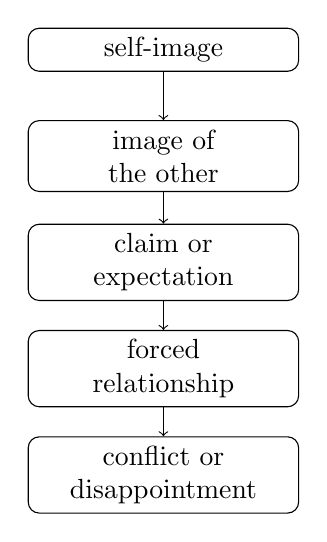
\begin{tikzpicture}[x=1cm,y=1cm]
\node[draw, rounded corners, text width=3.2cm, align=center] (a) at (0,0) {self-image};
\node[draw, rounded corners, text width=3.2cm, align=center] (b) at (0,-1.35) {image of\\the other};
\node[draw, rounded corners, text width=3.2cm, align=center] (c) at (0,-2.70) {claim or\\expectation};
\node[draw, rounded corners, text width=3.2cm, align=center] (d) at (0,-4.05) {forced\\relationship};
\node[draw, rounded corners, text width=3.2cm, align=center] (e) at (0,-5.40) {conflict or\\disappointment};

\draw[->] (a) -- (b);
\draw[->] (b) -- (c);
\draw[->] (c) -- (d);
\draw[->] (d) -- (e);
\end{tikzpicture}
\caption{A transcript-backed reconstruction of relationship under image. No validated screenshot supplies an original board diagram for this point.}
\end{figure}

\section{Energy, Seriousness, And The Refusal To Delegate}

The lecture then asks a practical question: can one watch the image in the office, factory, home, and all the other places where relationship occurs? This brings in energy. Krishnamurti explicitly says that he is not using energy in a scientific sense. It means vitality, seriousness, drive, the capacity not to be dissipated.

The first examples are ordinary: drink, smoke, useless chatter, moving from pub to pub. These are not introduced as sins. They are examples of wastage once the importance of relationship has been seen. The order matters. The dialogue does not begin by imposing discipline; it says that if relationship is seen as of the greatest importance, waste is seen as waste.

\begin{equation}
\text{seeing the importance of relationship}
\;\longrightarrow\;
\text{seeing what wastes energy}.
\end{equation}

But the lecture does not stay with obvious waste. It turns to a subtler image: someone else will do it for me. Or, still deeper, I cannot do it myself. This is one of the most important loops in the dialogue. The image of incapacity may seek escape; the escape then confirms the image.

\begin{align}
\text{I cannot do it myself}
&\longrightarrow \text{escape or dependence} \\
&\longrightarrow \text{confirmation of incapacity} \\
&\longrightarrow \text{renewed demand for rescue}.
\end{align}

This is why the dialogue insists that nobody can do this for another. Another may point, question, or live differently, but imitation does not transform one's relationship. Right relationship begins with seeing the utter importance of the matter and the responsibility that follows from seeing it.

The phrase ``you are the world'' enters here. It should not be turned into a slogan. The meaning is concrete: the basic structure of suffering, anxiety, confusion, fear, hope, and deception is shared. One may go to India, Europe, or America and find different surfaces but the same essential human movement. Responsibility is not private self-improvement; it is responsibility within a universal structure.

\subsection{Question \& Answer}

\paragraph{Question.}
Can another person bring about right relationship for me?

\paragraph{Answer.}
No. If another person lives beautifully, I may admire, imitate, depend, or resist, but my relationship remains as before unless I see the image operating in myself. The wish that another will do it for me is itself an image, and the image of incapacity feeds the very disorder it wants another to solve.

\section{Consciousness As Interrelated Images}

At this point the dialogue gathers the examples into a larger claim. As long as there is image, pleasant or unpleasant, put together by thought, there is no right relationship. Without right relationship, life loses value. Then the next step becomes unavoidable: my consciousness is filled with these images.

The formulation is deliberately approximate:

\begin{equation}
\text{consciousness as known}
\;\approx\;
\{\text{interrelated images centered on the self}\}.
\end{equation}

The approximation sign is important. We are not defining consciousness in a technical system. We are marking the dialogue's observation that the content of ordinary consciousness is largely made of images: what I am, what I was, what I should become, what I deserve, what you did, what I fear, what I hope, what will make me secure.

The images are interrelated, not isolated. Their center is the self-image. The self is the one to be protected, improved, comforted, vindicated, and continued. Therefore to end image-making is not a minor adjustment; it calls into question consciousness as one knows it.

At this point the ordinary question appears: how am I to do it? The dialogue refuses that question in its usual form because the ``how'' quietly reinstates the one who will perform the method.

\begin{proposition}
In the dialogue's logic, the demand for a method can rebuild the image-maker.
\end{proposition}

\begin{proof}
To ask ``how shall I do it?'' is to imply a procedure. A procedure implies a self who will apply it, measure progress, compare results, and arrive. But that self is not outside the image-process; it is the image-maker itself. Therefore the demand for a method can carry forward the very center it proposes to end.
\end{proof}

As a schematic sequence:

\begin{align}
\text{how shall I do it?}
&\longrightarrow \text{method or system} \\
&\longrightarrow \text{me applying the method} \\
&\longrightarrow \text{image-maker restored}.
\end{align}

\subsection{Question \& Answer}

\paragraph{Question.}
Why does asking ``how do I end image-making?'' recreate the image-maker?

\paragraph{Answer.}
Because the word ``how'' usually contains the ``me'' implicitly. It may not say ``me'' aloud, but it assumes a center that will practice, apply, accumulate, and succeed. The lecture does not reject clarity or action; it rejects the hidden return of the self-image as the doer of transformation.

\section{Pleasure, Hurt, And Registration}

The dialogue now slows down and gives us its clearest worked example. My wife calls me an idiot. The event is registered in the brain. Thought takes it over. Memory enters. The image I have about myself is hurt. The same machinery works with flattery. Praise is registered, thought takes it over, and the image becomes pleasure.

The update rule is:

\begin{equation}
\text{event}
\;\longrightarrow\;
\text{registration}
\;\longrightarrow\;
\text{thought/memory}
\;\longrightarrow\;
\text{image}
\;\longrightarrow\;
\text{hurt or pleasure}.
\end{equation}

This is the strongest diagrammatic candidate in the lecture because the transcript itself supplies the sequence. The diagram below is an editorial reconstruction, not an extracted frame.

\begin{figure}
\centering
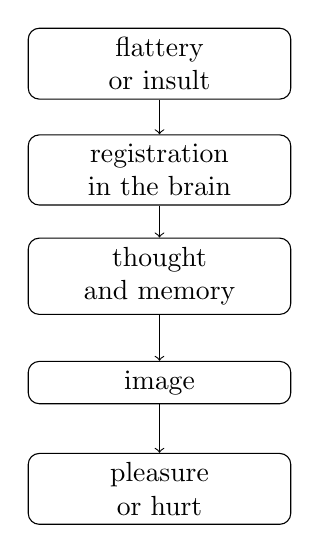
\begin{tikzpicture}[x=1cm,y=1cm]
\node[draw, rounded corners, text width=3.1cm, align=center] (a) at (0,0) {flattery\\or insult};
\node[draw, rounded corners, text width=3.1cm, align=center] (b) at (0,-1.35) {registration\\in the brain};
\node[draw, rounded corners, text width=3.1cm, align=center] (c) at (0,-2.70) {thought\\and memory};
\node[draw, rounded corners, text width=3.1cm, align=center] (d) at (0,-4.05) {image};
\node[draw, rounded corners, text width=3.1cm, align=center] (e) at (0,-5.40) {pleasure\\or hurt};

\draw[->] (a) -- (b);
\draw[->] (b) -- (c);
\draw[->] (c) -- (d);
\draw[->] (d) -- (e);
\end{tikzpicture}
\caption{The image-making chain reconstructed from the insult and flattery passage.}
\end{figure}

\paragraph{Worked example.}
Take the insulting sentence, ``You are an idiot.'' The point is not merely that sound is heard. The insult is registered, then thought and memory take possession of the registration. The old image of oneself as competent, respectable, intelligent, or deserving recognition is struck. The image, with insult as its new content, is hurt.

\begin{enumerate}
\item An event occurs: insult.
\item The brain registers the event.
\item Thought and memory take over the registration.
\item The self-image is activated or reinforced.
\item With insult as content, the image is hurt.
\end{enumerate}

For flattery the machinery is the same and the content changes.

\begin{table}
\centering
\begin{tabular}{|p{0.36\linewidth}|p{0.36\linewidth}|}
\hline
\textbf{Flattery} & \textbf{Insult} \\
\hline
Registered by the brain & Registered by the brain \\
\hline
Thought and memory take it over & Thought and memory take it over \\
\hline
Image expands as pleasure & Image contracts as hurt \\
\hline
The self-image is gratified & The self-image is wounded \\
\hline
\end{tabular}
\caption{Flattery and insult as two contents of the same image-process.}
\end{table}

In the compact notation of the chapter:

\begin{equation}
\text{flattery} \longrightarrow \text{image-as-pleasure},
\qquad
\text{insult} \longrightarrow \text{image-as-hurt}.
\end{equation}

And more generally:

\begin{equation}
\text{pleasure} \sim \text{hurt}.
\end{equation}

The symbol \(\sim\) does not mean that pleasure and hurt feel identical. It means that in this passage they belong to the same image-process. Flattery and insult are different contents; the machinery of registration, thought, memory, and self-image is shared.

The next obstacle is whether past hurts and future hurts must be handled separately. The dialogue says no. A remembered hurt can operate like a fresh insult; a future hurt is already conditioned by past reaction. Therefore the inquiry is not to divide hurt by date, but to look at the image in its general structure.

\begin{equation}
\text{past hurt}
\not\perp
\text{future hurt}.
\end{equation}

This is again shorthand, not a theorem. It means: do not treat past and future hurt as separate principles. The process is one movement of image.

\section{The Observer Is The Observed}

Now the central question appears. If image is the structure, how am I to look at it? The difficulty is immediate: I may already be looking with another image. I may look with the image that I must suppress it. I may look with the image that right relationship will give me a beautiful life. I may look with the image that I am serious, intelligent, or capable. The real question is whether the observer is different from that which is observed.

The ordinary assumption says yes. There is an observer here and an image there. The dialogue does not dismiss that assumption too quickly. It says: let us look at it. If the observer is different from the observed, there is an interval. In that interval time enters; in time there is adjustment, escape, substitution, and conflict.

\begin{equation}
\text{observer} \neq \text{observed}
\;\longrightarrow\;
\text{interval}
\;\longrightarrow\;
\text{time}
\;\longrightarrow\;
\text{conflict}.
\end{equation}

Bohm then recalls a distinction about reality. We should keep it narrow, because the lecture does not build a full metaphysical system. The distinction is only used to examine the apparent solidity of the self.

\begin{table}
\centering
\begin{tabular}{|p{0.28\linewidth}|p{0.46\linewidth}|}
\hline
\textbf{Kind of reality} & \textbf{Use in the dialogue} \\
\hline
Thought-made reality & Nations, churches, images, and constructions put together by thought. \\
\hline
Reality sustained by thought & A reality that continues only through thought's maintenance and reference. \\
\hline
Reality independent of thought & Nature is used as the example of what is not put together by thought. \\
\hline
\end{tabular}
\caption{A cautious reconstruction of the reality distinction used to question the apparent independence of the self.}
\end{table}

Ordinarily, we feel that the self is a reality independent of thought. The self appears to be the observer who possesses thought and looks at images. The dialogue asks whether this is so. The observer is reconstructed as the past: memories, experiences, accumulated incidents, old becoming, and projection into the future. The ``me'' that appears to look at the past is itself made of the past.

\begin{equation}
\text{past memories}
\;\longrightarrow\;
\text{me as image}
\;\longrightarrow\;
\text{projected future}.
\end{equation}

This is psychological time. It is not clock time. It is the movement by which the image of myself at three, five, ten, seventeen, and now is strung together as though a substantial observer had traveled through a sequence. The lecture asks whether that movement is an actuality or an image. Intellectual agreement is not enough; the point is whether there is immediate perception of the fact.

The conjuring-trick analogy sharpens the matter. Before the trick is seen through, one seems to perceive a woman being cut in half. When the trick is seen, one does not merely improve the old perception; one sees that the old perception depended on missing the essential points. Likewise, as long as the observer is assumed to stand outside the image, the image has power. When the observer is seen as part of the image-process, the question changes.

\begin{equation}
\text{observer} = \text{observed}.
\end{equation}

This identity is not algebra. It is the dialogue's central shorthand. The observer is the past, the movement of thought, the maker of image. If that observer is not separate from the image, then the image-maker has no independent standing.

\begin{figure}
\centering
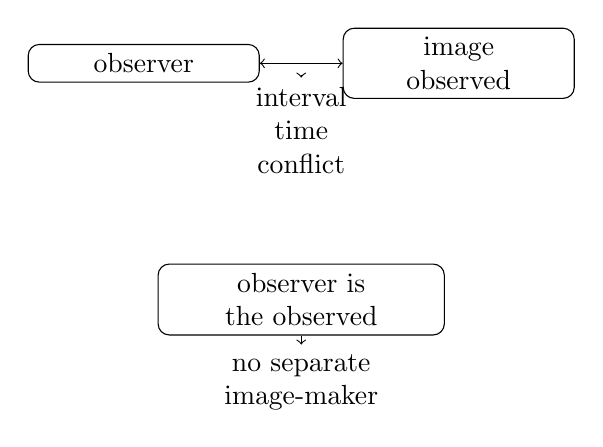
\begin{tikzpicture}[x=1cm,y=1cm]
\node[draw, rounded corners, text width=2.7cm, align=center] (o1) at (-2.0,0) {observer};
\node[draw, rounded corners, text width=2.7cm, align=center] (i1) at (2.0,0) {image\\observed};
\node[text width=3.2cm, align=center] (t1) at (0,-0.85) {interval\\time\\conflict};
\draw[<->] (o1) -- (i1);
\draw[->] (0,-0.15) -- (t1);

\node[draw, rounded corners, text width=3.4cm, align=center] (o2) at (0,-3.0) {observer is\\the observed};
\node[text width=3.5cm, align=center] (n2) at (0,-4.05) {no separate\\image-maker};
\draw[->] (o2) -- (n2);
\end{tikzpicture}
\caption{The observer division reconstructed as a two-stage conceptual diagram: separation first, then the seeing-through of separation.}
\end{figure}

\subsection{Question \& Answer}

\paragraph{Question.}
Is the observer different from the image being observed?

\paragraph{Answer.}
The dialogue says no. The observer appears different because thought presents the self as though it were an independent reality looking at its own contents. But the observer is made of memory, past experience, preference, fear, and image. Therefore the observer is not outside the observed image. The observer is the observed.

The point can be turned around in two parallel forms:

\begin{equation}
\text{no thinker apart from thought},
\qquad
\text{no image-maker apart from image}.
\end{equation}

If there is no observer in the old sense, the instruction ``look at the image'' changes meaning. It is no longer one fragment controlling another. It is the seeing of the image-process without a separate center claiming to look.

\section{When Image-Making Ends}

After the observer and observed are brought together, the dialogue raises a residual objection: what about hidden images? Are there deep, underground images that one must unearth one by one? This is where the line about there being no unconscious must be handled with care. The dialogue is not making a general clinical doctrine. It is following its own local logic: if the observer is the observed, the one who would dig out hidden images is not standing outside the field.

The strong formulation is:

\begin{equation}
\text{observer} = \text{observed}
\;\longrightarrow\;
\text{no separate image-maker}
\;\longrightarrow\;
\text{image-making ends}.
\end{equation}

This is the point at which consciousness as known is said to undergo transformation. The content of consciousness, as the dialogue has described it, is filled with the things of thought: sorrow, fear, pleasure, despair, anxiety, attachment, detachment, hope, confusion, and the deep agony involved in all that. In such a state, relationship is impossible because image is always between.

The final turn opens toward meditation. The question is not what practice to adopt. Krishnamurti explicitly places practices, gurus, and religious identities inside the same danger if they operate within the old field of image and image-maker. The question is more radical: when there is no movement of thought as image-making, when psychological time ends, what takes place?

\begin{equation}
\text{thought as image-making ends}
\;\Longrightarrow\;
\text{consciousness as known is transformed}.
\end{equation}

The arrow is cautious. It marks the direction of the dialogue, not a mechanical proof. Thought still has its right place in knowledge and practical functioning. What ends is thought as the maker of self, image, fear, pursuit of pleasure, anxiety, division, and turmoil.

\subsection{Question \& Answer}

\paragraph{Question.}
Is this the death of the self, and what does the lecture leave open?

\paragraph{Answer.}
The dialogue calls it the death of the self, but it resists reducing that phrase to destruction. It is the ending of the image-making center. What remains is not presented as an experience, because experience would imply an experiencer. The lecture stops at the question: when thought as psychological time ends, what takes place?

\section{Summary}

The lecture unfolds in a strict order. It begins with the question of radical transformation and refuses to let scientific authority answer it. It brings the question down to ordinary life and chooses relationship as the field where the problem can be seen. Relationship then reveals image: self-image, image of the other, entitlement, security, pleasure, and hurt.

The middle of the lecture makes the structure explicit. Energy means seriousness and vitality, not a scientific quantity. Dependency on another is exposed as another image. Consciousness as known is described as interrelated images centered on the self. Asking for a method restores the self as the one who will perform transformation. Insult and flattery show the machinery of registration, thought, memory, image, hurt, and pleasure. Past and future hurt are not separate principles; they belong to one image-process.

The decisive movement is the observer and the observed. The observer first appears separate, but this separation creates interval, time, and conflict. The observer is then seen as past, thought, memory, and image. If the observer is the observed, the image-maker has no separate standing. The lecture ends at the edge of meditation: when thought as image-making time ends, what remains? It does not package an answer. It leaves the question open, serious, and alive.